% Created by tikzDevice version 0.10.1 on 2018-01-22 11:53:54
% !TEX encoding = UTF-8 Unicode
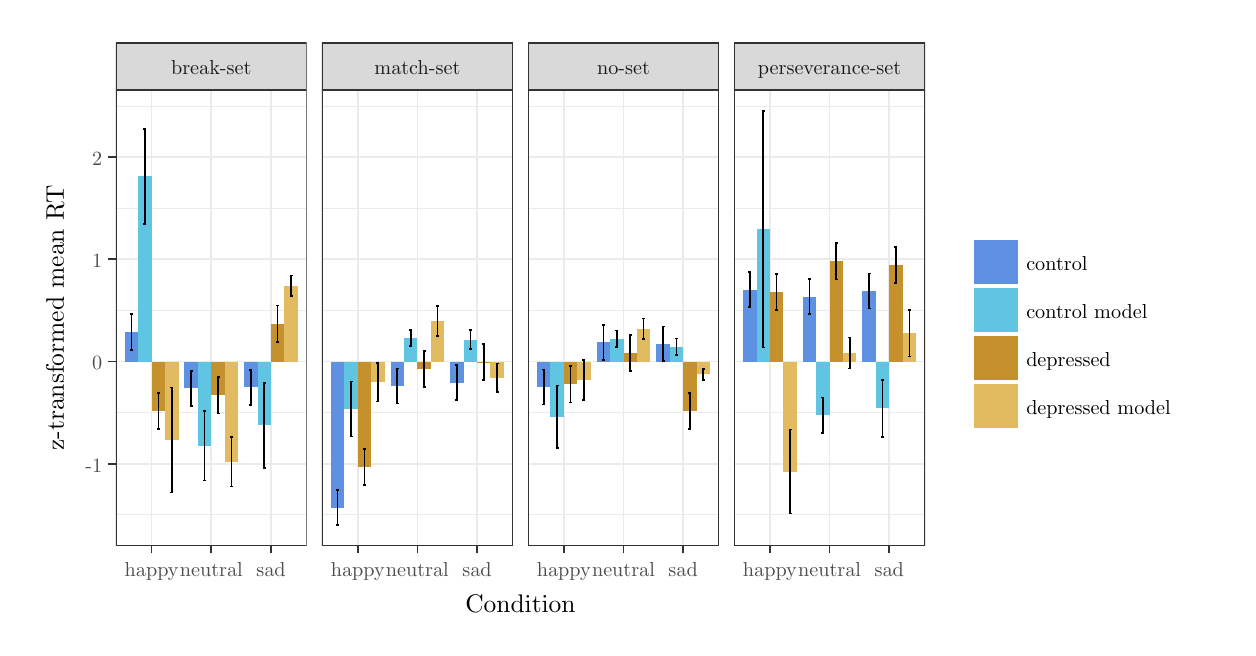
\begin{tikzpicture}[x=1pt,y=1pt]
\definecolor{fillColor}{RGB}{255,255,255}
\path[use as bounding box,fill=fillColor,fill opacity=0.00] (0,0) rectangle (433.62,216.81);
\begin{scope}
\path[clip] (  0.00,  0.00) rectangle (433.62,216.81);
\definecolor{drawColor}{RGB}{255,255,255}
\definecolor{fillColor}{RGB}{255,255,255}

\path[draw=drawColor,line width= 0.6pt,line join=round,line cap=round,fill=fillColor] (  0.00,  0.00) rectangle (433.62,216.81);
\end{scope}
\begin{scope}
\path[clip] ( 31.87, 29.59) rectangle (100.84,194.25);
\definecolor{fillColor}{RGB}{255,255,255}

\path[fill=fillColor] ( 31.87, 29.59) rectangle (100.84,194.25);
\definecolor{drawColor}{gray}{0.92}

\path[draw=drawColor,line width= 0.3pt,line join=round] ( 31.87, 40.75) --
	(100.84, 40.75);

\path[draw=drawColor,line width= 0.3pt,line join=round] ( 31.87, 77.69) --
	(100.84, 77.69);

\path[draw=drawColor,line width= 0.3pt,line join=round] ( 31.87,114.63) --
	(100.84,114.63);

\path[draw=drawColor,line width= 0.3pt,line join=round] ( 31.87,151.57) --
	(100.84,151.57);

\path[draw=drawColor,line width= 0.3pt,line join=round] ( 31.87,188.51) --
	(100.84,188.51);

\path[draw=drawColor,line width= 0.6pt,line join=round] ( 31.87, 59.22) --
	(100.84, 59.22);

\path[draw=drawColor,line width= 0.6pt,line join=round] ( 31.87, 96.16) --
	(100.84, 96.16);

\path[draw=drawColor,line width= 0.6pt,line join=round] ( 31.87,133.10) --
	(100.84,133.10);

\path[draw=drawColor,line width= 0.6pt,line join=round] ( 31.87,170.04) --
	(100.84,170.04);

\path[draw=drawColor,line width= 0.6pt,line join=round] ( 44.80, 29.59) --
	( 44.80,194.25);

\path[draw=drawColor,line width= 0.6pt,line join=round] ( 66.36, 29.59) --
	( 66.36,194.25);

\path[draw=drawColor,line width= 0.6pt,line join=round] ( 87.91, 29.59) --
	( 87.91,194.25);
\definecolor{fillColor}{RGB}{226,186,95}

\path[fill=fillColor] ( 49.65, 67.79) rectangle ( 54.50, 96.16);
\definecolor{fillColor}{RGB}{196,145,45}

\path[fill=fillColor] ( 44.80, 78.35) rectangle ( 49.65, 96.16);
\definecolor{fillColor}{RGB}{95,197,226}

\path[fill=fillColor] ( 39.95, 96.16) rectangle ( 44.80,163.03);
\definecolor{fillColor}{RGB}{95,145,226}

\path[fill=fillColor] ( 35.10, 96.16) rectangle ( 39.95,106.76);
\definecolor{fillColor}{RGB}{226,186,95}

\path[fill=fillColor] ( 71.21, 59.97) rectangle ( 76.06, 96.16);
\definecolor{fillColor}{RGB}{196,145,45}

\path[fill=fillColor] ( 66.36, 83.97) rectangle ( 71.21, 96.16);
\definecolor{fillColor}{RGB}{95,197,226}

\path[fill=fillColor] ( 61.51, 65.69) rectangle ( 66.36, 96.16);
\definecolor{fillColor}{RGB}{95,145,226}

\path[fill=fillColor] ( 56.66, 86.44) rectangle ( 61.51, 96.16);
\definecolor{fillColor}{RGB}{226,186,95}

\path[fill=fillColor] ( 92.76, 96.16) rectangle ( 97.61,123.55);
\definecolor{fillColor}{RGB}{196,145,45}

\path[fill=fillColor] ( 87.91, 96.16) rectangle ( 92.76,109.86);
\definecolor{fillColor}{RGB}{95,197,226}

\path[fill=fillColor] ( 83.06, 73.09) rectangle ( 87.91, 96.16);
\definecolor{fillColor}{RGB}{95,145,226}

\path[fill=fillColor] ( 78.21, 86.86) rectangle ( 83.06, 96.16);
\definecolor{drawColor}{RGB}{0,0,0}

\path[draw=drawColor,line width= 0.6pt,line join=round] ( 51.54, 86.77) --
	( 52.62, 86.77);

\path[draw=drawColor,line width= 0.6pt,line join=round] ( 52.08, 86.77) --
	( 52.08, 48.82);

\path[draw=drawColor,line width= 0.6pt,line join=round] ( 51.54, 48.82) --
	( 52.62, 48.82);

\path[draw=drawColor,line width= 0.6pt,line join=round] ( 46.69, 84.91) --
	( 47.77, 84.91);

\path[draw=drawColor,line width= 0.6pt,line join=round] ( 47.23, 84.91) --
	( 47.23, 71.79);

\path[draw=drawColor,line width= 0.6pt,line join=round] ( 46.69, 71.79) --
	( 47.77, 71.79);

\path[draw=drawColor,line width= 0.6pt,line join=round] ( 41.84,180.08) --
	( 42.92,180.08);

\path[draw=drawColor,line width= 0.6pt,line join=round] ( 42.38,180.08) --
	( 42.38,145.98);

\path[draw=drawColor,line width= 0.6pt,line join=round] ( 41.84,145.98) --
	( 42.92,145.98);

\path[draw=drawColor,line width= 0.6pt,line join=round] ( 36.99,113.24) --
	( 38.07,113.24);

\path[draw=drawColor,line width= 0.6pt,line join=round] ( 37.53,113.24) --
	( 37.53,100.29);

\path[draw=drawColor,line width= 0.6pt,line join=round] ( 36.99,100.29) --
	( 38.07,100.29);

\path[draw=drawColor,line width= 0.6pt,line join=round] ( 73.09, 68.88) --
	( 74.17, 68.88);

\path[draw=drawColor,line width= 0.6pt,line join=round] ( 73.63, 68.88) --
	( 73.63, 51.05);

\path[draw=drawColor,line width= 0.6pt,line join=round] ( 73.09, 51.05) --
	( 74.17, 51.05);

\path[draw=drawColor,line width= 0.6pt,line join=round] ( 68.24, 90.50) --
	( 69.32, 90.50);

\path[draw=drawColor,line width= 0.6pt,line join=round] ( 68.78, 90.50) --
	( 68.78, 77.43);

\path[draw=drawColor,line width= 0.6pt,line join=round] ( 68.24, 77.43) --
	( 69.32, 77.43);

\path[draw=drawColor,line width= 0.6pt,line join=round] ( 63.39, 78.21) --
	( 64.47, 78.21);

\path[draw=drawColor,line width= 0.6pt,line join=round] ( 63.93, 78.21) --
	( 63.93, 53.18);

\path[draw=drawColor,line width= 0.6pt,line join=round] ( 63.39, 53.18) --
	( 64.47, 53.18);

\path[draw=drawColor,line width= 0.6pt,line join=round] ( 58.54, 92.75) --
	( 59.62, 92.75);

\path[draw=drawColor,line width= 0.6pt,line join=round] ( 59.08, 92.75) --
	( 59.08, 80.13);

\path[draw=drawColor,line width= 0.6pt,line join=round] ( 58.54, 80.13) --
	( 59.62, 80.13);

\path[draw=drawColor,line width= 0.6pt,line join=round] ( 94.65,127.28) --
	( 95.72,127.28);

\path[draw=drawColor,line width= 0.6pt,line join=round] ( 95.18,127.28) --
	( 95.18,119.81);

\path[draw=drawColor,line width= 0.6pt,line join=round] ( 94.65,119.81) --
	( 95.72,119.81);

\path[draw=drawColor,line width= 0.6pt,line join=round] ( 89.80,116.42) --
	( 90.87,116.42);

\path[draw=drawColor,line width= 0.6pt,line join=round] ( 90.33,116.42) --
	( 90.33,103.31);

\path[draw=drawColor,line width= 0.6pt,line join=round] ( 89.80,103.31) --
	( 90.87,103.31);

\path[draw=drawColor,line width= 0.6pt,line join=round] ( 84.95, 88.37) --
	( 86.02, 88.37);

\path[draw=drawColor,line width= 0.6pt,line join=round] ( 85.48, 88.37) --
	( 85.48, 57.80);

\path[draw=drawColor,line width= 0.6pt,line join=round] ( 84.95, 57.80) --
	( 86.02, 57.80);

\path[draw=drawColor,line width= 0.6pt,line join=round] ( 80.10, 93.17) --
	( 81.17, 93.17);

\path[draw=drawColor,line width= 0.6pt,line join=round] ( 80.64, 93.17) --
	( 80.64, 80.55);

\path[draw=drawColor,line width= 0.6pt,line join=round] ( 80.10, 80.55) --
	( 81.17, 80.55);
\definecolor{drawColor}{gray}{0.20}

\path[draw=drawColor,line width= 0.6pt,line join=round,line cap=round] ( 31.87, 29.59) rectangle (100.84,194.25);
\end{scope}
\begin{scope}
\path[clip] (106.34, 29.59) rectangle (175.31,194.25);
\definecolor{fillColor}{RGB}{255,255,255}

\path[fill=fillColor] (106.34, 29.59) rectangle (175.31,194.25);
\definecolor{drawColor}{gray}{0.92}

\path[draw=drawColor,line width= 0.3pt,line join=round] (106.34, 40.75) --
	(175.31, 40.75);

\path[draw=drawColor,line width= 0.3pt,line join=round] (106.34, 77.69) --
	(175.31, 77.69);

\path[draw=drawColor,line width= 0.3pt,line join=round] (106.34,114.63) --
	(175.31,114.63);

\path[draw=drawColor,line width= 0.3pt,line join=round] (106.34,151.57) --
	(175.31,151.57);

\path[draw=drawColor,line width= 0.3pt,line join=round] (106.34,188.51) --
	(175.31,188.51);

\path[draw=drawColor,line width= 0.6pt,line join=round] (106.34, 59.22) --
	(175.31, 59.22);

\path[draw=drawColor,line width= 0.6pt,line join=round] (106.34, 96.16) --
	(175.31, 96.16);

\path[draw=drawColor,line width= 0.6pt,line join=round] (106.34,133.10) --
	(175.31,133.10);

\path[draw=drawColor,line width= 0.6pt,line join=round] (106.34,170.04) --
	(175.31,170.04);

\path[draw=drawColor,line width= 0.6pt,line join=round] (119.27, 29.59) --
	(119.27,194.25);

\path[draw=drawColor,line width= 0.6pt,line join=round] (140.83, 29.59) --
	(140.83,194.25);

\path[draw=drawColor,line width= 0.6pt,line join=round] (162.38, 29.59) --
	(162.38,194.25);
\definecolor{fillColor}{RGB}{226,186,95}

\path[fill=fillColor] (124.12, 88.68) rectangle (128.97, 96.16);
\definecolor{fillColor}{RGB}{196,145,45}

\path[fill=fillColor] (119.27, 58.11) rectangle (124.12, 96.16);
\definecolor{fillColor}{RGB}{95,197,226}

\path[fill=fillColor] (114.42, 79.00) rectangle (119.27, 96.16);
\definecolor{fillColor}{RGB}{95,145,226}

\path[fill=fillColor] (109.57, 43.40) rectangle (114.42, 96.16);
\definecolor{fillColor}{RGB}{226,186,95}

\path[fill=fillColor] (145.68, 96.16) rectangle (150.53,110.81);
\definecolor{fillColor}{RGB}{196,145,45}

\path[fill=fillColor] (140.83, 93.48) rectangle (145.68, 96.16);
\definecolor{fillColor}{RGB}{95,197,226}

\path[fill=fillColor] (135.98, 96.16) rectangle (140.83,104.69);
\definecolor{fillColor}{RGB}{95,145,226}

\path[fill=fillColor] (131.13, 87.32) rectangle (135.98, 96.16);
\definecolor{fillColor}{RGB}{226,186,95}

\path[fill=fillColor] (167.23, 90.25) rectangle (172.08, 96.16);
\definecolor{fillColor}{RGB}{196,145,45}

\path[fill=fillColor] (162.38, 96.03) rectangle (167.23, 96.16);
\definecolor{fillColor}{RGB}{95,197,226}

\path[fill=fillColor] (157.53, 96.16) rectangle (162.38,104.07);
\definecolor{fillColor}{RGB}{95,145,226}

\path[fill=fillColor] (152.68, 88.53) rectangle (157.53, 96.16);
\definecolor{drawColor}{RGB}{0,0,0}

\path[draw=drawColor,line width= 0.6pt,line join=round] (126.01, 95.60) --
	(127.09, 95.60);

\path[draw=drawColor,line width= 0.6pt,line join=round] (126.55, 95.60) --
	(126.55, 81.75);

\path[draw=drawColor,line width= 0.6pt,line join=round] (126.01, 81.75) --
	(127.09, 81.75);

\path[draw=drawColor,line width= 0.6pt,line join=round] (121.16, 64.65) --
	(122.24, 64.65);

\path[draw=drawColor,line width= 0.6pt,line join=round] (121.70, 64.65) --
	(121.70, 51.57);

\path[draw=drawColor,line width= 0.6pt,line join=round] (121.16, 51.57) --
	(122.24, 51.57);

\path[draw=drawColor,line width= 0.6pt,line join=round] (116.31, 88.91) --
	(117.39, 88.91);

\path[draw=drawColor,line width= 0.6pt,line join=round] (116.85, 88.91) --
	(116.85, 69.08);

\path[draw=drawColor,line width= 0.6pt,line join=round] (116.31, 69.08) --
	(117.39, 69.08);

\path[draw=drawColor,line width= 0.6pt,line join=round] (111.46, 49.73) --
	(112.54, 49.73);

\path[draw=drawColor,line width= 0.6pt,line join=round] (112.00, 49.73) --
	(112.00, 37.07);

\path[draw=drawColor,line width= 0.6pt,line join=round] (111.46, 37.07) --
	(112.54, 37.07);

\path[draw=drawColor,line width= 0.6pt,line join=round] (147.56,116.22) --
	(148.64,116.22);

\path[draw=drawColor,line width= 0.6pt,line join=round] (148.10,116.22) --
	(148.10,105.41);

\path[draw=drawColor,line width= 0.6pt,line join=round] (147.56,105.41) --
	(148.64,105.41);

\path[draw=drawColor,line width= 0.6pt,line join=round] (142.71,100.02) --
	(143.79,100.02);

\path[draw=drawColor,line width= 0.6pt,line join=round] (143.25,100.02) --
	(143.25, 86.94);

\path[draw=drawColor,line width= 0.6pt,line join=round] (142.71, 86.94) --
	(143.79, 86.94);

\path[draw=drawColor,line width= 0.6pt,line join=round] (137.86,107.49) --
	(138.94,107.49);

\path[draw=drawColor,line width= 0.6pt,line join=round] (138.40,107.49) --
	(138.40,101.89);

\path[draw=drawColor,line width= 0.6pt,line join=round] (137.86,101.89) --
	(138.94,101.89);

\path[draw=drawColor,line width= 0.6pt,line join=round] (133.01, 93.63) --
	(134.09, 93.63);

\path[draw=drawColor,line width= 0.6pt,line join=round] (133.55, 93.63) --
	(133.55, 81.01);

\path[draw=drawColor,line width= 0.6pt,line join=round] (133.01, 81.01) --
	(134.09, 81.01);

\path[draw=drawColor,line width= 0.6pt,line join=round] (169.12, 95.43) --
	(170.19, 95.43);

\path[draw=drawColor,line width= 0.6pt,line join=round] (169.65, 95.43) --
	(169.65, 85.07);

\path[draw=drawColor,line width= 0.6pt,line join=round] (169.12, 85.07) --
	(170.19, 85.07);

\path[draw=drawColor,line width= 0.6pt,line join=round] (164.27,102.57) --
	(165.34,102.57);

\path[draw=drawColor,line width= 0.6pt,line join=round] (164.80,102.57) --
	(164.80, 89.50);

\path[draw=drawColor,line width= 0.6pt,line join=round] (164.27, 89.50) --
	(165.34, 89.50);

\path[draw=drawColor,line width= 0.6pt,line join=round] (159.42,107.52) --
	(160.49,107.52);

\path[draw=drawColor,line width= 0.6pt,line join=round] (159.96,107.52) --
	(159.96,100.63);

\path[draw=drawColor,line width= 0.6pt,line join=round] (159.42,100.63) --
	(160.49,100.63);

\path[draw=drawColor,line width= 0.6pt,line join=round] (154.57, 94.84) --
	(155.64, 94.84);

\path[draw=drawColor,line width= 0.6pt,line join=round] (155.11, 94.84) --
	(155.11, 82.23);

\path[draw=drawColor,line width= 0.6pt,line join=round] (154.57, 82.23) --
	(155.64, 82.23);
\definecolor{drawColor}{gray}{0.20}

\path[draw=drawColor,line width= 0.6pt,line join=round,line cap=round] (106.34, 29.59) rectangle (175.31,194.25);
\end{scope}
\begin{scope}
\path[clip] (180.81, 29.59) rectangle (249.78,194.25);
\definecolor{fillColor}{RGB}{255,255,255}

\path[fill=fillColor] (180.81, 29.59) rectangle (249.78,194.25);
\definecolor{drawColor}{gray}{0.92}

\path[draw=drawColor,line width= 0.3pt,line join=round] (180.81, 40.75) --
	(249.78, 40.75);

\path[draw=drawColor,line width= 0.3pt,line join=round] (180.81, 77.69) --
	(249.78, 77.69);

\path[draw=drawColor,line width= 0.3pt,line join=round] (180.81,114.63) --
	(249.78,114.63);

\path[draw=drawColor,line width= 0.3pt,line join=round] (180.81,151.57) --
	(249.78,151.57);

\path[draw=drawColor,line width= 0.3pt,line join=round] (180.81,188.51) --
	(249.78,188.51);

\path[draw=drawColor,line width= 0.6pt,line join=round] (180.81, 59.22) --
	(249.78, 59.22);

\path[draw=drawColor,line width= 0.6pt,line join=round] (180.81, 96.16) --
	(249.78, 96.16);

\path[draw=drawColor,line width= 0.6pt,line join=round] (180.81,133.10) --
	(249.78,133.10);

\path[draw=drawColor,line width= 0.6pt,line join=round] (180.81,170.04) --
	(249.78,170.04);

\path[draw=drawColor,line width= 0.6pt,line join=round] (193.74, 29.59) --
	(193.74,194.25);

\path[draw=drawColor,line width= 0.6pt,line join=round] (215.30, 29.59) --
	(215.30,194.25);

\path[draw=drawColor,line width= 0.6pt,line join=round] (236.85, 29.59) --
	(236.85,194.25);
\definecolor{fillColor}{RGB}{226,186,95}

\path[fill=fillColor] (198.59, 89.49) rectangle (203.44, 96.16);
\definecolor{fillColor}{RGB}{196,145,45}

\path[fill=fillColor] (193.74, 87.95) rectangle (198.59, 96.16);
\definecolor{fillColor}{RGB}{95,197,226}

\path[fill=fillColor] (188.89, 76.29) rectangle (193.74, 96.16);
\definecolor{fillColor}{RGB}{95,145,226}

\path[fill=fillColor] (184.05, 86.98) rectangle (188.89, 96.16);
\definecolor{fillColor}{RGB}{226,186,95}

\path[fill=fillColor] (220.15, 96.16) rectangle (225.00,108.03);
\definecolor{fillColor}{RGB}{196,145,45}

\path[fill=fillColor] (215.30, 96.16) rectangle (220.15, 99.26);
\definecolor{fillColor}{RGB}{95,197,226}

\path[fill=fillColor] (210.45, 96.16) rectangle (215.30,104.41);
\definecolor{fillColor}{RGB}{95,145,226}

\path[fill=fillColor] (205.60, 96.16) rectangle (210.45,103.12);
\definecolor{fillColor}{RGB}{226,186,95}

\path[fill=fillColor] (241.70, 91.49) rectangle (246.55, 96.16);
\definecolor{fillColor}{RGB}{196,145,45}

\path[fill=fillColor] (236.85, 78.22) rectangle (241.70, 96.16);
\definecolor{fillColor}{RGB}{95,197,226}

\path[fill=fillColor] (232.00, 96.16) rectangle (236.85,101.49);
\definecolor{fillColor}{RGB}{95,145,226}

\path[fill=fillColor] (227.15, 96.16) rectangle (232.00,102.57);
\definecolor{drawColor}{RGB}{0,0,0}

\path[draw=drawColor,line width= 0.6pt,line join=round] (200.48, 96.68) --
	(201.56, 96.68);

\path[draw=drawColor,line width= 0.6pt,line join=round] (201.02, 96.68) --
	(201.02, 82.31);

\path[draw=drawColor,line width= 0.6pt,line join=round] (200.48, 82.31) --
	(201.56, 82.31);

\path[draw=drawColor,line width= 0.6pt,line join=round] (195.63, 94.48) --
	(196.71, 94.48);

\path[draw=drawColor,line width= 0.6pt,line join=round] (196.17, 94.48) --
	(196.17, 81.41);

\path[draw=drawColor,line width= 0.6pt,line join=round] (195.63, 81.41) --
	(196.71, 81.41);

\path[draw=drawColor,line width= 0.6pt,line join=round] (190.78, 87.54) --
	(191.86, 87.54);

\path[draw=drawColor,line width= 0.6pt,line join=round] (191.32, 87.54) --
	(191.32, 65.04);

\path[draw=drawColor,line width= 0.6pt,line join=round] (190.78, 65.04) --
	(191.86, 65.04);

\path[draw=drawColor,line width= 0.6pt,line join=round] (185.93, 93.31) --
	(187.01, 93.31);

\path[draw=drawColor,line width= 0.6pt,line join=round] (186.47, 93.31) --
	(186.47, 80.66);

\path[draw=drawColor,line width= 0.6pt,line join=round] (185.93, 80.66) --
	(187.01, 80.66);

\path[draw=drawColor,line width= 0.6pt,line join=round] (222.03,111.75) --
	(223.11,111.75);

\path[draw=drawColor,line width= 0.6pt,line join=round] (222.57,111.75) --
	(222.57,104.30);

\path[draw=drawColor,line width= 0.6pt,line join=round] (222.03,104.30) --
	(223.11,104.30);

\path[draw=drawColor,line width= 0.6pt,line join=round] (217.18,105.82) --
	(218.26,105.82);

\path[draw=drawColor,line width= 0.6pt,line join=round] (217.72,105.82) --
	(217.72, 92.70);

\path[draw=drawColor,line width= 0.6pt,line join=round] (217.18, 92.70) --
	(218.26, 92.70);

\path[draw=drawColor,line width= 0.6pt,line join=round] (212.33,107.35) --
	(213.41,107.35);

\path[draw=drawColor,line width= 0.6pt,line join=round] (212.87,107.35) --
	(212.87,101.46);

\path[draw=drawColor,line width= 0.6pt,line join=round] (212.33,101.46) --
	(213.41,101.46);

\path[draw=drawColor,line width= 0.6pt,line join=round] (207.48,109.42) --
	(208.56,109.42);

\path[draw=drawColor,line width= 0.6pt,line join=round] (208.02,109.42) --
	(208.02, 96.81);

\path[draw=drawColor,line width= 0.6pt,line join=round] (207.48, 96.81) --
	(208.56, 96.81);

\path[draw=drawColor,line width= 0.6pt,line join=round] (243.59, 93.42) --
	(244.66, 93.42);

\path[draw=drawColor,line width= 0.6pt,line join=round] (244.12, 93.42) --
	(244.12, 89.56);

\path[draw=drawColor,line width= 0.6pt,line join=round] (243.59, 89.56) --
	(244.66, 89.56);

\path[draw=drawColor,line width= 0.6pt,line join=round] (238.74, 84.76) --
	(239.81, 84.76);

\path[draw=drawColor,line width= 0.6pt,line join=round] (239.28, 84.76) --
	(239.28, 71.69);

\path[draw=drawColor,line width= 0.6pt,line join=round] (238.74, 71.69) --
	(239.81, 71.69);

\path[draw=drawColor,line width= 0.6pt,line join=round] (233.89,104.48) --
	(234.96,104.48);

\path[draw=drawColor,line width= 0.6pt,line join=round] (234.43,104.48) --
	(234.43, 98.50);

\path[draw=drawColor,line width= 0.6pt,line join=round] (233.89, 98.50) --
	(234.96, 98.50);

\path[draw=drawColor,line width= 0.6pt,line join=round] (229.04,108.88) --
	(230.12,108.88);

\path[draw=drawColor,line width= 0.6pt,line join=round] (229.58,108.88) --
	(229.58, 96.27);

\path[draw=drawColor,line width= 0.6pt,line join=round] (229.04, 96.27) --
	(230.12, 96.27);
\definecolor{drawColor}{gray}{0.20}

\path[draw=drawColor,line width= 0.6pt,line join=round,line cap=round] (180.81, 29.59) rectangle (249.78,194.25);
\end{scope}
\begin{scope}
\path[clip] (255.28, 29.59) rectangle (324.25,194.25);
\definecolor{fillColor}{RGB}{255,255,255}

\path[fill=fillColor] (255.28, 29.59) rectangle (324.25,194.25);
\definecolor{drawColor}{gray}{0.92}

\path[draw=drawColor,line width= 0.3pt,line join=round] (255.28, 40.75) --
	(324.25, 40.75);

\path[draw=drawColor,line width= 0.3pt,line join=round] (255.28, 77.69) --
	(324.25, 77.69);

\path[draw=drawColor,line width= 0.3pt,line join=round] (255.28,114.63) --
	(324.25,114.63);

\path[draw=drawColor,line width= 0.3pt,line join=round] (255.28,151.57) --
	(324.25,151.57);

\path[draw=drawColor,line width= 0.3pt,line join=round] (255.28,188.51) --
	(324.25,188.51);

\path[draw=drawColor,line width= 0.6pt,line join=round] (255.28, 59.22) --
	(324.25, 59.22);

\path[draw=drawColor,line width= 0.6pt,line join=round] (255.28, 96.16) --
	(324.25, 96.16);

\path[draw=drawColor,line width= 0.6pt,line join=round] (255.28,133.10) --
	(324.25,133.10);

\path[draw=drawColor,line width= 0.6pt,line join=round] (255.28,170.04) --
	(324.25,170.04);

\path[draw=drawColor,line width= 0.6pt,line join=round] (268.21, 29.59) --
	(268.21,194.25);

\path[draw=drawColor,line width= 0.6pt,line join=round] (289.77, 29.59) --
	(289.77,194.25);

\path[draw=drawColor,line width= 0.6pt,line join=round] (311.32, 29.59) --
	(311.32,194.25);
\definecolor{fillColor}{RGB}{226,186,95}

\path[fill=fillColor] (273.06, 56.42) rectangle (277.91, 96.16);
\definecolor{fillColor}{RGB}{196,145,45}

\path[fill=fillColor] (268.21, 96.16) rectangle (273.06,121.35);
\definecolor{fillColor}{RGB}{95,197,226}

\path[fill=fillColor] (263.37, 96.16) rectangle (268.21,143.98);
\definecolor{fillColor}{RGB}{95,145,226}

\path[fill=fillColor] (258.52, 96.16) rectangle (263.37,122.14);
\definecolor{fillColor}{RGB}{226,186,95}

\path[fill=fillColor] (294.62, 96.16) rectangle (299.47, 99.25);
\definecolor{fillColor}{RGB}{196,145,45}

\path[fill=fillColor] (289.77, 96.16) rectangle (294.62,132.41);
\definecolor{fillColor}{RGB}{95,197,226}

\path[fill=fillColor] (284.92, 76.83) rectangle (289.77, 96.16);
\definecolor{fillColor}{RGB}{95,145,226}

\path[fill=fillColor] (280.07, 96.16) rectangle (284.92,119.59);
\definecolor{fillColor}{RGB}{226,186,95}

\path[fill=fillColor] (316.17, 96.16) rectangle (321.02,106.42);
\definecolor{fillColor}{RGB}{196,145,45}

\path[fill=fillColor] (311.32, 96.16) rectangle (316.17,130.99);
\definecolor{fillColor}{RGB}{95,197,226}

\path[fill=fillColor] (306.47, 79.25) rectangle (311.32, 96.16);
\definecolor{fillColor}{RGB}{95,145,226}

\path[fill=fillColor] (301.62, 96.16) rectangle (306.47,121.68);
\definecolor{drawColor}{RGB}{0,0,0}

\path[draw=drawColor,line width= 0.6pt,line join=round] (274.95, 71.63) --
	(276.03, 71.63);

\path[draw=drawColor,line width= 0.6pt,line join=round] (275.49, 71.63) --
	(275.49, 41.20);

\path[draw=drawColor,line width= 0.6pt,line join=round] (274.95, 41.20) --
	(276.03, 41.20);

\path[draw=drawColor,line width= 0.6pt,line join=round] (270.10,127.88) --
	(271.18,127.88);

\path[draw=drawColor,line width= 0.6pt,line join=round] (270.64,127.88) --
	(270.64,114.81);

\path[draw=drawColor,line width= 0.6pt,line join=round] (270.10,114.81) --
	(271.18,114.81);

\path[draw=drawColor,line width= 0.6pt,line join=round] (265.25,186.76) --
	(266.33,186.76);

\path[draw=drawColor,line width= 0.6pt,line join=round] (265.79,186.76) --
	(265.79,101.19);

\path[draw=drawColor,line width= 0.6pt,line join=round] (265.25,101.19) --
	(266.33,101.19);

\path[draw=drawColor,line width= 0.6pt,line join=round] (260.40,128.45) --
	(261.48,128.45);

\path[draw=drawColor,line width= 0.6pt,line join=round] (260.94,128.45) --
	(260.94,115.83);

\path[draw=drawColor,line width= 0.6pt,line join=round] (260.40,115.83) --
	(261.48,115.83);

\path[draw=drawColor,line width= 0.6pt,line join=round] (296.50,104.84) --
	(297.58,104.84);

\path[draw=drawColor,line width= 0.6pt,line join=round] (297.04,104.84) --
	(297.04, 93.66);

\path[draw=drawColor,line width= 0.6pt,line join=round] (296.50, 93.66) --
	(297.58, 93.66);

\path[draw=drawColor,line width= 0.6pt,line join=round] (291.65,138.95) --
	(292.73,138.95);

\path[draw=drawColor,line width= 0.6pt,line join=round] (292.19,138.95) --
	(292.19,125.87);

\path[draw=drawColor,line width= 0.6pt,line join=round] (291.65,125.87) --
	(292.73,125.87);

\path[draw=drawColor,line width= 0.6pt,line join=round] (286.80, 83.20) --
	(287.88, 83.20);

\path[draw=drawColor,line width= 0.6pt,line join=round] (287.34, 83.20) --
	(287.34, 70.46);

\path[draw=drawColor,line width= 0.6pt,line join=round] (286.80, 70.46) --
	(287.88, 70.46);

\path[draw=drawColor,line width= 0.6pt,line join=round] (281.95,125.89) --
	(283.03,125.89);

\path[draw=drawColor,line width= 0.6pt,line join=round] (282.49,125.89) --
	(282.49,113.28);

\path[draw=drawColor,line width= 0.6pt,line join=round] (281.95,113.28) --
	(283.03,113.28);

\path[draw=drawColor,line width= 0.6pt,line join=round] (318.06,114.85) --
	(319.13,114.85);

\path[draw=drawColor,line width= 0.6pt,line join=round] (318.60,114.85) --
	(318.60, 97.98);

\path[draw=drawColor,line width= 0.6pt,line join=round] (318.06, 97.98) --
	(319.13, 97.98);

\path[draw=drawColor,line width= 0.6pt,line join=round] (313.21,137.52) --
	(314.28,137.52);

\path[draw=drawColor,line width= 0.6pt,line join=round] (313.75,137.52) --
	(313.75,124.45);

\path[draw=drawColor,line width= 0.6pt,line join=round] (313.21,124.45) --
	(314.28,124.45);

\path[draw=drawColor,line width= 0.6pt,line join=round] (308.36, 89.53) --
	(309.44, 89.53);

\path[draw=drawColor,line width= 0.6pt,line join=round] (308.90, 89.53) --
	(308.90, 68.96);

\path[draw=drawColor,line width= 0.6pt,line join=round] (308.36, 68.96) --
	(309.44, 68.96);

\path[draw=drawColor,line width= 0.6pt,line join=round] (303.51,127.99) --
	(304.59,127.99);

\path[draw=drawColor,line width= 0.6pt,line join=round] (304.05,127.99) --
	(304.05,115.37);

\path[draw=drawColor,line width= 0.6pt,line join=round] (303.51,115.37) --
	(304.59,115.37);
\definecolor{drawColor}{gray}{0.20}

\path[draw=drawColor,line width= 0.6pt,line join=round,line cap=round] (255.28, 29.59) rectangle (324.25,194.25);
\end{scope}
\begin{scope}
\path[clip] ( 31.87,194.25) rectangle (100.84,211.31);
\definecolor{drawColor}{gray}{0.20}
\definecolor{fillColor}{gray}{0.85}

\path[draw=drawColor,line width= 0.6pt,line join=round,line cap=round,fill=fillColor] ( 31.87,194.25) rectangle (100.84,211.31);
\definecolor{drawColor}{gray}{0.10}

\node[text=drawColor,anchor=base,inner sep=0pt, outer sep=0pt, scale=  0.73] at ( 66.36,199.75) {break-set};
\end{scope}
\begin{scope}
\path[clip] (106.34,194.25) rectangle (175.31,211.31);
\definecolor{drawColor}{gray}{0.20}
\definecolor{fillColor}{gray}{0.85}

\path[draw=drawColor,line width= 0.6pt,line join=round,line cap=round,fill=fillColor] (106.34,194.25) rectangle (175.31,211.31);
\definecolor{drawColor}{gray}{0.10}

\node[text=drawColor,anchor=base,inner sep=0pt, outer sep=0pt, scale=  0.73] at (140.83,199.75) {match-set};
\end{scope}
\begin{scope}
\path[clip] (180.81,194.25) rectangle (249.78,211.31);
\definecolor{drawColor}{gray}{0.20}
\definecolor{fillColor}{gray}{0.85}

\path[draw=drawColor,line width= 0.6pt,line join=round,line cap=round,fill=fillColor] (180.81,194.25) rectangle (249.78,211.31);
\definecolor{drawColor}{gray}{0.10}

\node[text=drawColor,anchor=base,inner sep=0pt, outer sep=0pt, scale=  0.73] at (215.30,199.75) {no-set};
\end{scope}
\begin{scope}
\path[clip] (255.28,194.25) rectangle (324.25,211.31);
\definecolor{drawColor}{gray}{0.20}
\definecolor{fillColor}{gray}{0.85}

\path[draw=drawColor,line width= 0.6pt,line join=round,line cap=round,fill=fillColor] (255.28,194.25) rectangle (324.25,211.31);
\definecolor{drawColor}{gray}{0.10}

\node[text=drawColor,anchor=base,inner sep=0pt, outer sep=0pt, scale=  0.73] at (289.77,199.75) {perseverance-set};
\end{scope}
\begin{scope}
\path[clip] (  0.00,  0.00) rectangle (433.62,216.81);
\definecolor{drawColor}{gray}{0.20}

\path[draw=drawColor,line width= 0.6pt,line join=round] ( 44.80, 26.84) --
	( 44.80, 29.59);

\path[draw=drawColor,line width= 0.6pt,line join=round] ( 66.36, 26.84) --
	( 66.36, 29.59);

\path[draw=drawColor,line width= 0.6pt,line join=round] ( 87.91, 26.84) --
	( 87.91, 29.59);
\end{scope}
\begin{scope}
\path[clip] (  0.00,  0.00) rectangle (433.62,216.81);
\definecolor{drawColor}{gray}{0.30}

\node[text=drawColor,anchor=base,inner sep=0pt, outer sep=0pt, scale=  0.73] at ( 44.80, 18.58) {happy};

\node[text=drawColor,anchor=base,inner sep=0pt, outer sep=0pt, scale=  0.73] at ( 66.36, 18.58) {neutral};

\node[text=drawColor,anchor=base,inner sep=0pt, outer sep=0pt, scale=  0.73] at ( 87.91, 18.58) {sad};
\end{scope}
\begin{scope}
\path[clip] (  0.00,  0.00) rectangle (433.62,216.81);
\definecolor{drawColor}{gray}{0.20}

\path[draw=drawColor,line width= 0.6pt,line join=round] (119.27, 26.84) --
	(119.27, 29.59);

\path[draw=drawColor,line width= 0.6pt,line join=round] (140.83, 26.84) --
	(140.83, 29.59);

\path[draw=drawColor,line width= 0.6pt,line join=round] (162.38, 26.84) --
	(162.38, 29.59);
\end{scope}
\begin{scope}
\path[clip] (  0.00,  0.00) rectangle (433.62,216.81);
\definecolor{drawColor}{gray}{0.30}

\node[text=drawColor,anchor=base,inner sep=0pt, outer sep=0pt, scale=  0.73] at (119.27, 18.58) {happy};

\node[text=drawColor,anchor=base,inner sep=0pt, outer sep=0pt, scale=  0.73] at (140.83, 18.58) {neutral};

\node[text=drawColor,anchor=base,inner sep=0pt, outer sep=0pt, scale=  0.73] at (162.38, 18.58) {sad};
\end{scope}
\begin{scope}
\path[clip] (  0.00,  0.00) rectangle (433.62,216.81);
\definecolor{drawColor}{gray}{0.20}

\path[draw=drawColor,line width= 0.6pt,line join=round] (193.74, 26.84) --
	(193.74, 29.59);

\path[draw=drawColor,line width= 0.6pt,line join=round] (215.30, 26.84) --
	(215.30, 29.59);

\path[draw=drawColor,line width= 0.6pt,line join=round] (236.85, 26.84) --
	(236.85, 29.59);
\end{scope}
\begin{scope}
\path[clip] (  0.00,  0.00) rectangle (433.62,216.81);
\definecolor{drawColor}{gray}{0.30}

\node[text=drawColor,anchor=base,inner sep=0pt, outer sep=0pt, scale=  0.73] at (193.74, 18.58) {happy};

\node[text=drawColor,anchor=base,inner sep=0pt, outer sep=0pt, scale=  0.73] at (215.30, 18.58) {neutral};

\node[text=drawColor,anchor=base,inner sep=0pt, outer sep=0pt, scale=  0.73] at (236.85, 18.58) {sad};
\end{scope}
\begin{scope}
\path[clip] (  0.00,  0.00) rectangle (433.62,216.81);
\definecolor{drawColor}{gray}{0.20}

\path[draw=drawColor,line width= 0.6pt,line join=round] (268.21, 26.84) --
	(268.21, 29.59);

\path[draw=drawColor,line width= 0.6pt,line join=round] (289.77, 26.84) --
	(289.77, 29.59);

\path[draw=drawColor,line width= 0.6pt,line join=round] (311.32, 26.84) --
	(311.32, 29.59);
\end{scope}
\begin{scope}
\path[clip] (  0.00,  0.00) rectangle (433.62,216.81);
\definecolor{drawColor}{gray}{0.30}

\node[text=drawColor,anchor=base,inner sep=0pt, outer sep=0pt, scale=  0.73] at (268.21, 18.58) {happy};

\node[text=drawColor,anchor=base,inner sep=0pt, outer sep=0pt, scale=  0.73] at (289.77, 18.58) {neutral};

\node[text=drawColor,anchor=base,inner sep=0pt, outer sep=0pt, scale=  0.73] at (311.32, 18.58) {sad};
\end{scope}
\begin{scope}
\path[clip] (  0.00,  0.00) rectangle (433.62,216.81);
\definecolor{drawColor}{gray}{0.30}

\node[text=drawColor,anchor=base east,inner sep=0pt, outer sep=0pt, scale=  0.73] at ( 26.92, 56.19) {-1};

\node[text=drawColor,anchor=base east,inner sep=0pt, outer sep=0pt, scale=  0.73] at ( 26.92, 93.13) {0};

\node[text=drawColor,anchor=base east,inner sep=0pt, outer sep=0pt, scale=  0.73] at ( 26.92,130.07) {1};

\node[text=drawColor,anchor=base east,inner sep=0pt, outer sep=0pt, scale=  0.73] at ( 26.92,167.01) {2};
\end{scope}
\begin{scope}
\path[clip] (  0.00,  0.00) rectangle (433.62,216.81);
\definecolor{drawColor}{gray}{0.20}

\path[draw=drawColor,line width= 0.6pt,line join=round] ( 29.12, 59.22) --
	( 31.87, 59.22);

\path[draw=drawColor,line width= 0.6pt,line join=round] ( 29.12, 96.16) --
	( 31.87, 96.16);

\path[draw=drawColor,line width= 0.6pt,line join=round] ( 29.12,133.10) --
	( 31.87,133.10);

\path[draw=drawColor,line width= 0.6pt,line join=round] ( 29.12,170.04) --
	( 31.87,170.04);
\end{scope}
\begin{scope}
\path[clip] (  0.00,  0.00) rectangle (433.62,216.81);
\definecolor{drawColor}{RGB}{0,0,0}

\node[text=drawColor,anchor=base,inner sep=0pt, outer sep=0pt, scale=  0.92] at (178.06,  5.50) {Condition};
\end{scope}
\begin{scope}
\path[clip] (  0.00,  0.00) rectangle (433.62,216.81);
\definecolor{drawColor}{RGB}{0,0,0}

\node[text=drawColor,rotate= 90.00,anchor=base,inner sep=0pt, outer sep=0pt, scale=  0.92] at ( 13.08,111.92) {z-transformed mean RT};
\end{scope}
\begin{scope}
\path[clip] (  0.00,  0.00) rectangle (433.62,216.81);
\definecolor{fillColor}{RGB}{255,255,255}

\path[fill=fillColor] (335.63, 65.58) rectangle (428.12,158.25);
\end{scope}
\begin{scope}
\path[clip] (  0.00,  0.00) rectangle (433.62,216.81);
\definecolor{fillColor}{RGB}{255,255,255}

\path[fill=fillColor] (341.32,123.31) rectangle (358.67,140.65);
\end{scope}
\begin{scope}
\path[clip] (  0.00,  0.00) rectangle (433.62,216.81);
\definecolor{fillColor}{RGB}{95,145,226}

\path[fill=fillColor] (342.04,124.02) rectangle (357.96,139.94);
\end{scope}
\begin{scope}
\path[clip] (  0.00,  0.00) rectangle (433.62,216.81);
\definecolor{fillColor}{RGB}{255,255,255}

\path[fill=fillColor] (341.32,105.96) rectangle (358.67,123.31);
\end{scope}
\begin{scope}
\path[clip] (  0.00,  0.00) rectangle (433.62,216.81);
\definecolor{fillColor}{RGB}{95,197,226}

\path[fill=fillColor] (342.04,106.67) rectangle (357.96,122.60);
\end{scope}
\begin{scope}
\path[clip] (  0.00,  0.00) rectangle (433.62,216.81);
\definecolor{fillColor}{RGB}{255,255,255}

\path[fill=fillColor] (341.32, 88.62) rectangle (358.67,105.96);
\end{scope}
\begin{scope}
\path[clip] (  0.00,  0.00) rectangle (433.62,216.81);
\definecolor{fillColor}{RGB}{196,145,45}

\path[fill=fillColor] (342.04, 89.33) rectangle (357.96,105.25);
\end{scope}
\begin{scope}
\path[clip] (  0.00,  0.00) rectangle (433.62,216.81);
\definecolor{fillColor}{RGB}{255,255,255}

\path[fill=fillColor] (341.32, 71.27) rectangle (358.67, 88.62);
\end{scope}
\begin{scope}
\path[clip] (  0.00,  0.00) rectangle (433.62,216.81);
\definecolor{fillColor}{RGB}{226,186,95}

\path[fill=fillColor] (342.04, 71.98) rectangle (357.96, 87.91);
\end{scope}
\begin{scope}
\path[clip] (  0.00,  0.00) rectangle (433.62,216.81);
\definecolor{drawColor}{RGB}{0,0,0}

\node[text=drawColor,anchor=base west,inner sep=0pt, outer sep=0pt, scale=  0.73] at (360.84,128.95) {control};
\end{scope}
\begin{scope}
\path[clip] (  0.00,  0.00) rectangle (433.62,216.81);
\definecolor{drawColor}{RGB}{0,0,0}

\node[text=drawColor,anchor=base west,inner sep=0pt, outer sep=0pt, scale=  0.73] at (360.84,111.60) {control model};
\end{scope}
\begin{scope}
\path[clip] (  0.00,  0.00) rectangle (433.62,216.81);
\definecolor{drawColor}{RGB}{0,0,0}

\node[text=drawColor,anchor=base west,inner sep=0pt, outer sep=0pt, scale=  0.73] at (360.84, 94.26) {depressed};
\end{scope}
\begin{scope}
\path[clip] (  0.00,  0.00) rectangle (433.62,216.81);
\definecolor{drawColor}{RGB}{0,0,0}

\node[text=drawColor,anchor=base west,inner sep=0pt, outer sep=0pt, scale=  0.73] at (360.84, 76.91) {depressed model};
\end{scope}
\end{tikzpicture}
